\documentclass[11pt,a4paper]{article}
\usepackage[margin=2.15cm]{geometry}
\usepackage[T1]{fontenc}
\usepackage{lmodern,microtype}
\usepackage{amsmath,amssymb,graphicx,booktabs,tabularx,array}
\usepackage{caption,placeins,xcolor,hyperref,xurl,needspace}
\usepackage[round,authoryear]{natbib}
\hypersetup{colorlinks=true,linkcolor=blue!50!black,citecolor=blue!50!black,
 urlcolor=blue!50!black,pdftitle={A compact DF model for Omega Centauri embedded in dark matter},
 pdfauthor={oCen dm project notes}}
\graphicspath{{../plots/}}
\captionsetup{font=small,labelfont=bf,skip=6pt}
\setlength{\emergencystretch}{3em}
\setlength{\parskip}{3pt}
\clubpenalty=10000
\widowpenalty=10000
\newcommand{\dd}{\mathrm{d}}
\newcommand{\Msun}{\mathrm{M}_\odot}
\newcommand{\pc}{\,\mathrm{pc}}
\newcommand{\dm}{\mathrm{DM}}
\newcommand{\remn}{\mathrm{rem}}
\newcommand{\mnras}{MNRAS}
\newcommand{\apj}{ApJ}
\newcommand{\aap}{A\&A}
\newcommand{\aj}{AJ}
\newcommand{\apjl}{ApJL}
\title{\vspace{-1cm}A compact distribution-function model for\texorpdfstring{\\[3pt]$\omega$ Centauri embedded in dark matter}{ Omega Centauri embedded in dark matter}\\[6pt]
\large Model proposal, literature basis and validation programme}
\author{oCen\_dm project notes}
\date{23 September 2026}
\begin{document}
\maketitle

\begin{abstract}
We propose a distribution-function (DF) model to constrain the present-day
mass distribution of $\omega$ Centauri, allowing an extended DM halo and
concentrated stellar remnants alongside self-gravitating stars. The primary
spherical candidate is a regularized exponential stellar action DF with an
anisotropy transition, combined with prescribed dark density profiles. Its
five stellar parameters describe mass, action scale, envelope shape,
anisotropy amplitude and transition scale. A two-parameter halo sampled in
$\rho_\dm(20\pc)$ and scale radius, plus two remnant parameters, gives nine
physical coordinates before light normalization and observational nuisance
parameters. A generalized lowered-isothermal stellar DF in the same combined
potential is the required independent control. The original linear-action
exponential is retained only as an analytic precursor. Matched-tracer checks,
rotation and flattening tests are required before treating spherical fits as
final DM constraints. Both stellar families are now implemented. Initial
numerical controls test the contours, normalization, self-gravity and projected
moments; scientific recovery and model-comparison experiments remain to be done.
\end{abstract}

\section{Motivation and the physical problem}

\subsection{The target: Omega Centauri}

$\omega$ Centauri (NGC~5139) is one of the Milky Way's most massive globular
clusters. It contains chemically distinct stellar populations and exhibits
both rotation and flattening \citep{2017MNRAS.468.4429Z}. These properties
make it a more complex target than a spherical cluster with one uniform
stellar population. A proposed origin is the surviving nucleus of an
accreted dwarf galaxy whose outer body was removed by Galactic tides
\citep{2003MNRAS.346L..11B}. This scenario motivates testing for a surviving
DM component; it does not establish that the present cluster retains one.

We model the present-day surviving cluster, rather than reconstructing its
entire progenitor in the equilibrium fit. The observational inputs are its
surface-brightness profile and stellar kinematics: the existing project
dataset contains 89 dispersion measurements, comprising 21 radial and 21
tangential HST proper-motion bins, 29 MUSE line-of-sight bins, and nine radial
and nine tangential Gaia proper-motion bins. These are profile measurements,
not a count of individual stars. The initial calculation adopts $D=5.43$~kpc.
``Remnants'' here means unseen stellar remnants, such as white dwarfs,
neutron stars and stellar-mass black holes; their possible concentrated mass
component is distinct from an extended DM halo.

\subsection{Why use a stellar distribution function?}

Our scientific question is whether the measured light and stellar motions
of $\omega$ Centauri require an extended dark component, and which present-day
DM densities, especially $\rho_\dm(20\pc)$, they allow. A compact stellar
cluster embedded in DM can be dominated by stars near its centre while the
halo contributes at larger radii. Concentrated stellar remnants and orbital
anisotropy can also affect the measured dispersions. We need a model that
compares these possibilities using photometry, line-of-sight velocities,
and both proper-motion components together.

The Jeans fits provide useful baseline mass and anisotropy constraints.
They describe velocity moments, however, and a solution of the moment
equations need not correspond to a non-negative stellar phase-space
distribution. The purpose of the DF approach is to impose this stronger
stellar consistency condition: a positive equilibrium $f_\star$ generates
the stellar density and kinematics in the same gravitational potential.
We seek the simplest stellar family that passes independent recovery tests
and reproduces the data at their precision. Several freely mixed stellar
DFs may provide approximation power, but their necessity must be established
before interpreting their individual masses as physical populations.

This motivation does not require a DF for every gravitating component.
In our stationary, smooth-potential fit, the unobserved DM and remnant
velocities do not enter the stellar likelihood at fixed dark density.
The recommended starting point is therefore one positive stellar DF plus
parametrized dark density profiles, with stellar self-gravity retained.
Explicit dark DFs are a separate option for stronger equilibrium checks
and live N-body initial conditions. Comparing these two formulations is
the purpose of Section~\ref{sec:dark}; neither is assumed in advance to
give a definitive DM detection or upper limit.

\subsection{Scope of the first model}

We start with a spherical, time-independent, nonrotating equilibrium at the
adopted distance and with no central black hole. A BH is a subsequent
extension. The spherical, single-tracer description is a controlled baseline
for the actual rotating, flattened, multiple-population object; it is not a
claim that those observed features are absent. Their effects must be tested
before interpreting residuals as evidence for DM or another mass component.

We use AGAMA for actions, velocity integrals and gravitational potentials
\citep{2019MNRAS.482.1525V}. Both formulations in
Section~\ref{sec:dark} determine the stellar density from a positive DF and
include all mass components in Poisson's equation:
\begin{align}
 \rho_\star(\boldsymbol x)&=\int
 f_\star[\boldsymbol J(\boldsymbol x,\boldsymbol v;\Phi_{\rm tot})]\,\dd^3v,
 \label{eq:density}\\
 \nabla^2\Phi_{\rm ext}&=4\pi G(\rho_\star+\rho_\remn+\rho_\dm),
 \qquad
 \Phi_{\rm tot}=\Phi_{\rm ext}-\frac{GM_\bullet}{r}.
 \label{eq:poisson}
\end{align}
Here $\Phi_{\rm ext}$ is the potential of the extended mass components, not
an external Galactic field. The initial stage sets $M_\bullet=0$.
For the first stellar fit, $\rho_\dm$ and $\rho_\remn$ may be prescribed
density profiles. Giving them positive DFs is a stronger modelling choice,
not a prerequisite for evaluating the stellar likelihood.

\begin{figure}[htbp]
\centering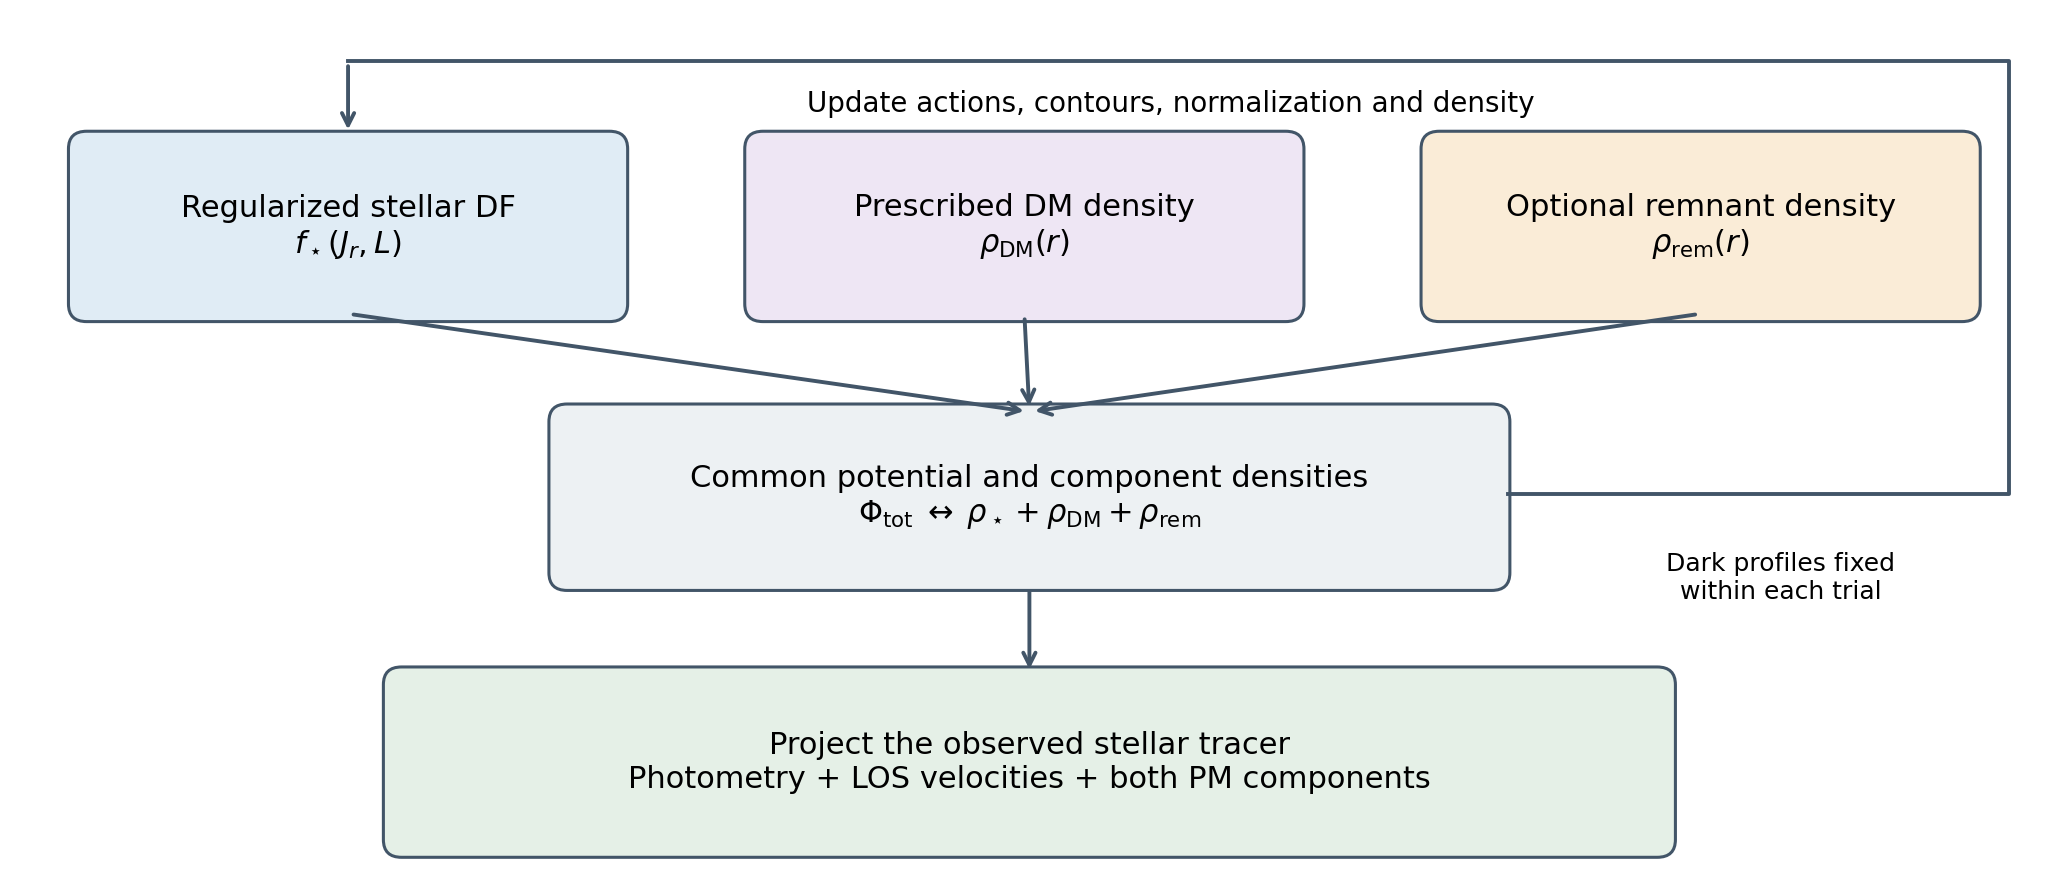
\includegraphics[width=.93\linewidth]{compact_df_proposal_architecture.png}
\caption{Recommended starting formulation: a positive stellar DF in the
combined potential of stars and prescribed dark density profiles. At each
trial, the stellar density and total potential are iterated together; the
dark profiles remain fixed during that iteration. Their parameters vary
between likelihood trials. Only the represented stellar tracer supplies the
observables. This is a model diagram, not a simulation result.}
\label{fig:architecture}
\end{figure}
\FloatBarrier

\section{A regularized exponential stellar DF}
\label{sec:stellar}

\subsection{Actions and the required low-angular-momentum limit}

In a spherical potential with $\Phi(\infty)=0$, define the specific energy,
angular momentum and radial action by
\begin{align}
 E&=\tfrac12 v^2+\Phi_{\rm tot}(r),\qquad L=|\boldsymbol r\times\boldsymbol v|,
 \\
 J_r(E,L)&=\frac{1}{\pi}\int_{r_{\rm peri}}^{r_{\rm apo}}
 \sqrt{2[E-\Phi_{\rm tot}(r)]-L^2/r^2}\,\dd r.
 \label{eq:jr}
\end{align}
Bound actions obey $J_r\geq0$ and $L=J_z+|J_\phi|$. They have units
pc\,km\,s$^{-1}$. The DF vanishes on unbound phase space.

For the smooth, finite-centre, no-BH baseline, regularity is an explicit
condition. At fixed $r$ and $v_r$, with $L=rv_t$, the radial-orbit limit gives
\begin{equation}
 \lim_{v_t\to0^+}\frac{\partial J_r}{\partial v_t}=-\frac r2,
 \qquad
 \lim_{v_t\to0^+}\frac{\partial f_\star}{\partial v_t}
 =r\lim_{L\to0^+}\left(\frac{\partial f_\star}{\partial L}
                  -\frac12\frac{\partial f_\star}{\partial J_r}\right).
 \label{eq:regularity-cancellation}
\end{equation}
Consequently the nonzero DF derivatives must satisfy
\begin{equation}
 \boxed{\lim_{L\to0^+}
 \frac{\partial f_\star/\partial J_r}{\partial f_\star/\partial L}=2.}
 \label{eq:regularity}
\end{equation}
This is the spherical smoothness constraint discussed by
\citet{2026MNRAS.549ag854B}. It concerns the local phase-space DF, not the
probability density of the \emph{magnitude} $v_t$, which includes a velocity
volume factor. A positive steady DF can still fail this smoothness test;
positivity, regularity and dynamical stability are separate requirements.
The finite-potential limit also covers the proposed $r^{-1}$ DM cusp, whose
central potential is finite. A point mass or a divergent central potential
requires a new limiting analysis: in a pure Kepler potential the derivative
ratio is one. We will also check the joint action-space origin, which is not
certified by a limit at fixed $J_r>0$ alone.

The precursor $f=F(J_r+\eta L)$ has derivative ratio $1/\eta$. Only
$\eta=1/2$ satisfies equation~\eqref{eq:regularity}; choosing that value does
not make the whole system isotropic at every radius. We retain this family
for analytic reproduction in Appendix~\ref{app:precursor}, not as the primary
inference model. Its envelope and orbital coefficients both change the
stellar density, so matching photometry cannot by itself determine its
anisotropy.

\subsection{Constant-DF contours for the reference model}
\label{sec:contours}

Retain the exponential envelope of \citet{2019MNRAS.488.2423P}, and adopt the
spherical contour construction of \citet{2026MNRAS.549ag854B}. At any
$(J_r,L)$, integrate
\begin{equation}
 \frac{\dd L}{\dd J_r}=-g(J_r,L),\qquad g>0,
 \label{eq:contour}
\end{equation}
towards decreasing $J_r$ until reaching $(0,L_c)$. The endpoint label
$L_c(J_r,L)$ defines the proposed DF:
\begin{equation}
 \boxed{f_\star(J_r,L)=A_\star
 \exp\left[-\left(\frac{L_c(J_r,L)}{J_{0,\star}}\right)^\alpha\right],
 \qquad J_{0,\star}>0,\quad\alpha>0.}
 \label{eq:stellar}
\end{equation}
Set $f_\star(0,0)=A_\star$ by continuity. Although positivity and finite
normalization require only $\alpha>0$, the implementation restricts
$\alpha>1/2$. In a harmonic core at $r=0$, $L_c\propto v^2$, so
$f(v)-f(0)\propto |v|^{2\alpha}$; this restriction makes the first velocity
derivative vanish at the joint origin. Away from the origin,
$L_c$ labels a constant-$f$ contour; it is not generally the angular
momentum of a circular orbit at the \emph{starting} orbit's energy.
Along a contour, $\dd f=0$ implies $f_{J_r}/f_L=g$, wherever the ratio is
defined. Thus building $g\to2$ at small $L$ enforces the required derivative
ratio directly.

For an exactly ergodic control in a specified spherical potential, use
\begin{equation}
 g_H(J_r,L)=\frac{\Omega_r(J_r,L)}{\Omega_t(J_r,L)},\qquad
 \Omega_r=\frac{\partial H}{\partial J_r},\quad
 \Omega_t=\frac{\partial H}{\partial L}.
 \label{eq:g-exact}
\end{equation}
Then the contours conserve energy. An economical approximation suggested
by the same construction is
\begin{equation}
 g_H^{\rm app}=\left[\frac12+c\left(\frac{\Omega}{\kappa}-\frac12\right)
                \right]^{-1},\qquad c=\frac{L}{L+J_r},
 \label{eq:g-approx}
\end{equation}
where $\Omega$ and $\kappa$ are the circular and radial epicycle frequencies.
For a concrete pointwise implementation, evaluate their ratio on the circular
orbit with angular momentum $\ell=L+1.4J_r$, at the current point along the
integration. This defines one vector field $g_H^{\rm app}(J_r,L)$ for all
contours. It is an approximation to test against equation~\eqref{eq:g-exact},
not a guarantee of exact isotropy. Positivity of $g$, smooth interpolation,
unique endpoints and convergence of the contour solver must be verified.

Introduce anisotropy with
\begin{equation}
 g(J_r,L)=g_H(J_r,L)
 \exp\left[-b(q)\sin\left(\frac{\pi c}{2}\right)\right],
 \qquad q=J_r+L.
 \label{eq:g-anisotropy}
\end{equation}
The choice of $q$ is part of this proposal. Positive $b$ favours radial
orbits relative to the ergodic reference; negative $b$ favours tangential
orbits. For bounded $b$, the sine makes $g\to g_H\to2$ at fixed $J_r>0$
as $L\to0$, regardless of anisotropy amplitude. With the approximate
$g_H$, these biases are relative to a nearly isotropic reference and must be
measured from the resulting moments.

The frequency map depends on the combined potential. Our reference
prescription rebuilds that map, the contour labels and the numerical
normalization as the trial potential changes. The converged model must
satisfy both the DF prescription and Poisson's equation. This is a
potential-dependent DF family, not an adiabatic evolution holding one
function of actions fixed. A frozen reference-frequency map would define a
different prescription and must be documented and tested separately.

\subsection{An anisotropy transition from the outset}
\label{sec:transition}

The primary candidate has
\begin{equation}
 b(q)=b_{\rm out}S(q/J_a),\qquad
 S(x)=\frac{x^n}{1+x^n},\qquad J_a>0,\qquad n=2\ \hbox{fixed}.
 \label{eq:b-one}
\end{equation}
The free stellar coordinates are $M_\star$, $J_{0,\star}$, $\alpha$,
$b_{\rm out}$ and $J_a$: five in total.
This replaces the free constant $\eta$; the net increase over the precursor
is one parameter, not two. At $b_{\rm out}=0$, $J_a$ is unidentifiable and
should be removed from the explicitly isotropic comparison.

The choice is motivated by the isotropic centre and outward radial bias in
the oMEGACat profiles \citep{2025ApJ...983...95H}, together with the
radial-to-tangential transition reported at larger radii in Gaia EDR3
\citep{2021MNRAS.505.5978V}. These samples probe different selections and
radial ranges. Neither their agreement nor a required turnover in our own
combined sample is assumed. If the matched-tracer data require a radial
intermediate region and tangential outskirts, test
\begin{equation}
 b(q)=b_1S(q/J_1)+(b_2-b_1)S(q/J_2),\qquad 0<J_1<J_2,
 \label{eq:b-two}
\end{equation}
with the same fixed $n$. This adds two coordinates relative to
$(b_{\rm out},J_a)$. A distinct intermediate plateau requires sufficiently
separated scales; merely imposing $J_2>J_1$ does not ensure it.

The functions $b(q)$ are orbital-weight prescriptions, not $\beta(r)$.
Orbits at one radius span many actions, and the potential itself changes
across the fit. An approximately isotropic core and a radial-to-tangential
profile must be demonstrated by the computed moments, not read off the signs
of $b_1,b_2$. Figure~\ref{fig:regularization} illustrates the inputs only.

\begin{figure}[htbp]
\centering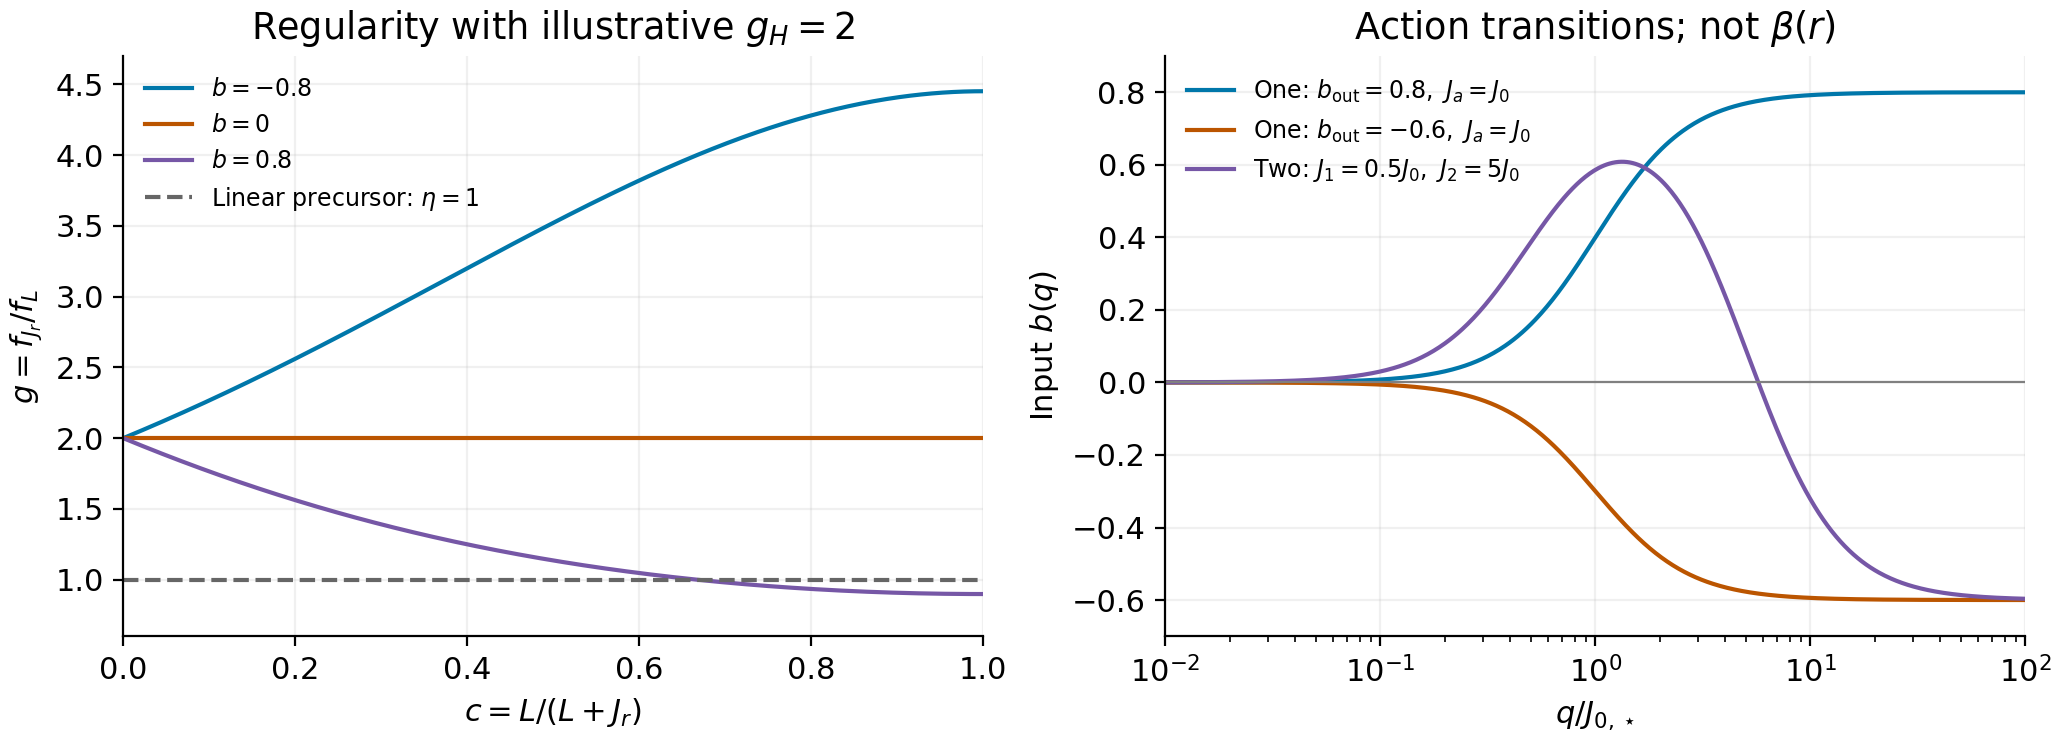
\includegraphics[width=\linewidth]{compact_df_proposal_regularization.png}
\caption{Dimensionless illustrations of the proposed orbital prescription.
Left: for the illustrative harmonic reference $g_H=2$, all bounded choices
of constant $b$ reach $g=2$ at $c=0$. The dashed line is the unregularized
$\eta=1$ precursor. Right: one- and two-transition input functions $b(q)$,
with action units set by $J_{0,\star}$ and $n=2$. These are not computed
$\beta(r)$ profiles, self-consistent equilibria or fits to data.}
\label{fig:regularization}
\end{figure}
\FloatBarrier

\subsection{Numerical normalization, mass and light}

The signed $J_\phi$ and positive $J_z$ integrals reduce to $2L\,\dd L$.
Normalize each trial with
\begin{equation}
 A_\star=\frac{M_\star}{(2\pi)^3\mathcal I_\star},\qquad
 \mathcal I_\star=2\int_0^\infty\!\dd J_r\int_0^\infty\!L\,\dd L\,
 \exp\left[-\left(\frac{L_c(J_r,L)}{J_{0,\star}}\right)^\alpha\right].
 \label{eq:norm}
\end{equation}
Use converged numerical quadrature, including the tail, rather than the
precursor's analytic normalization. A harmonic-reference, $b=0$ check gives
$L_c=L+2J_r$ and
$\mathcal I_\star=J_{0,\star}^3\Gamma(3/\alpha)/(2\alpha)$.
This also checks the action-scale conversion to the $\eta=1/2$ precursor.

Initially one effective stellar population has constant stellar
mass-to-light ratio $\Upsilon_\star$, so $j_\star=\rho_\star/\Upsilon_\star$.
$M_\star$ excludes any separately assigned remnant mass. The total M/L can
still vary through DM and remnants. The velocity moments give
\begin{equation}
 p_r=\int v_r^2f_\star\,\dd^3v,\qquad
 p_t=\tfrac12\int(v_\theta^2+v_\phi^2)f_\star\,\dd^3v,
 \qquad \beta(r)=1-p_t/p_r.
 \label{eq:beta}
\end{equation}
The contour construction separates envelope and orbital controls more
clearly, but changing $b(q)$ still changes the density. All stellar
parameters must be fitted jointly to photometry and kinematics. It does not
solve density--anisotropy covariance by construction. The one-tracer
approximation requires the checks in Section~\ref{sec:tracers} before a DM
interpretation.

\section{Dark components: density profiles or DFs}
\label{sec:dark}

\subsection{Stellar DF with prescribed dark densities: the starting model}
\label{sec:prescribed}

The observed stellar distribution constrains the total gravitational field.
Within the smooth, stationary approximation used here, the field depends on
the dark mass densities, not on the velocities of individual dark particles.
We therefore need not specify or fit a DM or remnant DF to calculate the
stellar observables. AGAMA explicitly supports density/potential components
without corresponding DFs \citep[section~5.2]{2019MNRAS.482.1525V}.

For the halo, sample the target density directly:
\begin{equation}
 \rho_\dm(r)=\rho_{20}
 \frac{h_\gamma(r/r_s)T(r/r_t)}
      {h_\gamma(20\pc/r_s)T(20\pc/r_t)},\qquad
 h_\gamma(x)=x^{-\gamma}(1+x)^{\gamma-3},\quad T(y)=e^{-y^2}.
 \label{eq:dark-density}
\end{equation}
This gives $\rho_\dm(20\pc)=\rho_{20}$ exactly. Compare a cored family
($\gamma=0$) and an NFW-like cusp ($\gamma=1$) separately, with sampling
coordinates $(\rho_{20},r_s)$ and positive $r_s,r_t$. The outer cutoff $r_t$
is a declared shape assumption, initially fixed within each run and varied
in sensitivity tests. It is not forced to equal the stellar boundary.
These are proposed reference profiles, not a claim that either is selected
by the data.

A concentrated remnant example is the Plummer density,
\begin{equation}
 \rho_\remn(r)=\frac{3M_\remn}{4\pi a_\remn^3}
       \left(1+\frac{r^2}{a_\remn^2}\right)^{-5/2},
 \qquad M_\remn\geq0,\quad a_\remn>0.
 \label{eq:remnant-density}
\end{equation}
Its normalization is a mass; the halo's normalization is a \emph{local
spatial density}. The corresponding potential of either spherical component,
with $\Phi_i(\infty)=0$, is
\begin{equation}
 \Phi_i(r)=-G\left[\frac{M_i(<r)}{r}
                   +4\pi\int_r^\infty s\rho_i(s)\dd s\right],
 \qquad M_i(<r)=4\pi\int_0^r s^2\rho_i(s)\dd s.
 \label{eq:dark-potential}
\end{equation}
Total halo mass is derived and may depend strongly on $r_t$ and extrapolation
beyond the stellar data. Sampling $\rho_{20}$ makes its prior explicit; a
change of coordinates alone does not remove prior sensitivity. A uniform
prior in $\rho_{20}$ and a uniform prior in $\log\rho_{20}$ are different
models. We must specify bounds and test that choice. The no-DM case is a
separate model with $\rho_{20}=0$, not the lower endpoint of a logarithmic
prior. Any model-averaged mass at zero also depends on model prior odds.
Outer density choices can affect bound-orbit actions and escape energies,
so their effect on $\rho_{20}$ must still be tested.

For each likelihood trial, hold the stellar DF parameters and dark density
parameters fixed. Compute $\Phi_\dm$ and $\Phi_\remn$, then iterate
equations~\eqref{eq:density}--\eqref{eq:poisson}: recalculate the stellar
actions and frequency map, rebuild and normalize the contour DF, and update
the stellar contribution to the total potential until convergence. This
additional DF update is required by the prescription in
Section~\ref{sec:contours}. This retains stellar self-gravity;
the cluster is not treated as a massless tracer. ``Prescribed'' means fixed
within this equilibrium calculation, not fixed across the parameter search.
The remnant component is optional, and the no-DM model sets $\rho_\dm=0$.

At fixed dark density profiles and stellar DF parameters, two different
dark orbital distributions produce the same smooth potential and stellar
likelihood. There is no direct information about those dark orbital
distributions in this likelihood. A chosen dark DF can link orbital
parameters to density and hence affect the stellar predictions indirectly;
that link is an additional model assumption. We recommend the prescribed
density formulation for the first compact-model fits.

\subsection{Positive DFs for all components: a stronger alternative}
\label{sec:dark-dfs}

The original proposal instead follows composite action-DF constructions
\citep{2018MNRAS.480..927P,2023MNRAS.520.1832B}. It replaces the prescribed
dark profiles by
\begin{equation}
 \rho_i(\boldsymbol x)=\int
 f_i[\boldsymbol J(\boldsymbol x,\boldsymbol v;\Phi_{\rm tot})]\,\dd^3v,
 \qquad i\in\{\dm,\remn\},
 \label{eq:dark-df-density}
\end{equation}
and recomputes all component densities as the common potential converges.
A non-negative DF is then required for every included extended component
in that potential. This certifies more than a stellar equilibrium in
prescribed dark gravity, although it still does not prove dynamical stability.

In this formulation the DM halo has its own mass, action scale, orbital prescription, core/cusp
choice and outer truncation. A useful notation for a positive normalized
component is
\begin{equation}
 f_i(\boldsymbol J)=\frac{M_i}{(2\pi)^3J_{0,i}^3\,\mathcal N_i}
 F_i\left(\frac{\boldsymbol J}{J_{0,i}};\boldsymbol\lambda_i\right),
 \qquad \mathcal N_i=\int F_i(\boldsymbol u;\boldsymbol\lambda_i)\dd^3u,
 \label{eq:generic}
\end{equation}
where $F_i\geq0$ and $0<\mathcal N_i<\infty$. The dimensionless shape
parameters $\boldsymbol\lambda_i$ must be stated for each model family.
This is a normalization convention, \emph{not yet a chosen halo or remnant
functional form}. The action double-power-law and cored/truncated constructions
of \citet{2015MNRAS.447.3060P,2018MNRAS.480..927P} provide candidates.
An action-space cusp parameter is not automatically the spatial density slope
in the final joint potential; the resulting $\rho_\dm(r)$ must be measured.

In either formulation the remnant component should be centrally concentrated but independent of
the extended halo. Its shape can initially be fixed while its mass and scale
vary. The halo must not be treated as another stellar mass bin with stellar
equipartition, nor forced to share the luminous truncation. Present-day
equilibrium does not imply a particular adiabatic formation history. Tidal
survival and stripping are separate dynamical constraints on acceptable
present-day configurations.

\subsection{Parameter budget and interpretation}

\begin{table}[htbp]
\centering\small
\caption{Physical coordinates for the primary spherical candidate, with one
anisotropy transition and prescribed dark densities. The fixed exponent
$n=2$, halo slope choice and outer cutoff are declared assumptions.}
\label{tab:parameters}
\begin{tabularx}{\linewidth}{lXr}
\toprule
Component & Free coordinates & Count\\
\midrule
Stars & $M_\star,J_{0,\star},\alpha,b_{\rm out},J_a$ & 5\\
Halo & $\rho_{20},r_s$ & 2\\
Remnants & $M_\remn,a_\remn$ & 2\\
\midrule
Stars + halo + remnants & & 9\\
Stars + halo only & & 7\\
Stars only & & 5\\
\bottomrule
\end{tabularx}
\end{table}

Light normalization, equivalently $\Upsilon_\star$ at fixed stellar mass,
is additional: the first row of totals becomes ten fitted coordinates if it
is the only extra parameter. Other observational nuisance parameters must
also be counted. The two-transition anisotropy law adds two coordinates;
releasing the halo cutoff adds one; a central BH adds $M_\bullet$ and requires
revisiting the stellar regularity prescription. Distance, flattening,
rotation and tracer extensions add their own parameters when introduced.
No-DM and no-remnant comparisons remove each absent component's irrelevant
scale parameters. There is no universal parameter count for every extension.

In the full dark-DF alternative, masses and action scales may replace the
halo/remnant density coordinates. Equal counts would not imply equal density
families or priors. Avoiding dark DFs simplifies the construction and avoids
unobserved orbital choices; it does not remove the degeneracy between
stellar mass, remnants and DM.

\subsection{When to construct dark DFs}
\label{sec:dark-validation}

The prescribed-density model guarantees neither that a dark profile has an
equilibrium orbital realization nor that the complete system is stable.
These are additional physical checks, distinct from fitting the stellar
data. For selected fitted models we can attempt a spherical density-to-DF
inversion in the \emph{combined} potential and test non-negativity and density
recovery. A successful isotropic inversion supplies one admissible DF. A
negative result rules out that isotropic realization; it does not by itself
exclude all anisotropic realizations of the same density. Any consistency
restriction imposed on the fit must state its orbital assumptions.

Live N-body experiments also need a velocity distribution for each sampled
dark component. Different admissible DFs at the same initial density can
respond differently to tides and heating. We can construct those DFs after
the stellar fit and assess that dependence in the dynamical experiments,
without adding unconstrained dark orbital parameters to the initial stellar
likelihood. An explicit dark-DF inference model remains an alternative if
we choose to impose that stronger equilibrium structure from the outset.

\section{Observable predictions and fitting}

\subsection{Tracer selection is a prerequisite for DM inference}
\label{sec:tracers}

Partial energy equipartition can make different stellar-mass samples have
different dispersions in the same potential. oMEGACat VI measures a radial
variation in this effect \citep{2025ApJ...983...95H}. HST, MUSE and Gaia
magnitude cuts, crowding cuts and spatial footprints therefore need explicit
comparison. Chemical populations are another possible distinction, but a
metallicity split is not automatically a stellar-mass split. The published
matched HST--MUSE comparison uses the same stars; we must establish which
selection is represented by each profile used here rather than assume that
all 89 bins have that property.

First audit each profile's stellar-mass/luminosity range, membership criteria,
error cuts, radial weights and rotation subtraction. Where catalogues allow,
construct kinematics for overlapping mass and population selections, and
fit those before combining unmatched profiles. If matching is impractical,
require a minimal two-tracer recovery test in a common potential. The tracer
DFs describe the selected populations; their number weights and light weights
must follow the selection, while stellar mass is counted only once in
Poisson's equation. Adding another freely weighted copy of the whole stellar
mass distribution would not perform this test.

Mocks should deliberately give the tracers different dispersions and spatial
profiles, then measure the false $\rho_{20}$ signal produced by forcing one
tracer. This tests confusion with anisotropy, M/L gradients and remnants.
A spherical DM result remains conditional until these controls establish its
sensitivity to the actual catalogue selections.


\subsection{Projection and sample weighting}

For the same effective stellar tracer, let $j=\rho_\star/\Upsilon_\star$ and
$\sigma_r^2=p_r/\rho_\star$. At projected radius $R$,
\begin{align}
 I(R)&=2\int_R^\infty\frac{j(r)r\,\dd r}{\sqrt{r^2-R^2}},\\
 I\sigma_{\rm LOS}^2(R)&=2\int_R^\infty
 \left(1-\beta\frac{R^2}{r^2}\right)
 \frac{j\sigma_r^2 r\,\dd r}{\sqrt{r^2-R^2}},\\
 I\sigma_{\rm PM,R}^2(R)&=2\int_R^\infty
 \left(1-\beta+\beta\frac{R^2}{r^2}\right)
 \frac{j\sigma_r^2 r\,\dd r}{\sqrt{r^2-R^2}},\\
 I\sigma_{\rm PM,T}^2(R)&=2\int_R^\infty
 (1-\beta)\frac{j\sigma_r^2 r\,\dd r}{\sqrt{r^2-R^2}}.
 \label{eq:projection}
\end{align}
These expressions are for the spherical nonrotating baseline. The observed
proper-motion dispersions follow by dividing velocities by
$4.74047\,D[\mathrm{kpc}]$ to obtain mas\,yr$^{-1}$.

For a catalogue with projected number density $\Sigma_a(R)$ and radial
selection $S_a(R)$, the model second moment in a complete annulus is
\begin{equation}
 \langle v_k^2\rangle_{a,b}=
 \frac{\int_{R_b^-}^{R_b^+}2\pi R\,S_a(R)\Sigma_a(R)
               \langle v_k^2\rangle_a(R)\dd R}
      {\int_{R_b^-}^{R_b^+}2\pi R\,S_a(R)\Sigma_a(R)\dd R}.
 \label{eq:annulus}
\end{equation}
The bin dispersion is the square root of the averaged variance, rather than
the average of the local dispersion. Actual spatial footprints and existing
bin kernels must be retained. Integrated light and a star-count-selected
kinematic sample need not weight stellar populations identically. The
single-tracer assumption is therefore explicit and must be checked for the
HST, MUSE and Gaia samples.

In a future discrete-data likelihood, the DF is marginalized over unmeasured
coordinates and convolved with velocity errors. Selection and contamination
are part of that probability model. Conditional velocity likelihoods can be
useful under specified selection assumptions
\citep{2026ApJ..1002...71V}; their cancellation of spatial selection is not
universal. Rotation also requires matching each data product's treatment of
mean streaming, not simply substituting raw second moments for dispersions.

\subsection{Inference targets}

The primary derived quantities are
\begin{equation}
 \rho_{\dm,20}\equiv\rho_\dm(20\pc),\qquad
 M_{\rm tot}(<20\pc)=4\pi\int_0^{20\pc}
 (\rho_\star+\rho_\remn+\rho_\dm)r^2\dd r+M_\bullet.
\end{equation}
The stellar/DM decomposition can be uncertain even when total enclosed mass
is well determined. Posterior uncertainties and sensitivity to halo shapes,
stellar M/L assumptions and anisotropy must accompany any inferred density.
The total outer halo mass is a different, extrapolation-sensitive quantity.

Where the errors are calibrated Gaussian measurements, a joint fit uses the
appropriate covariance in $-2\ln\mathcal L=\boldsymbol r^T C^{-1}\boldsymbol r
+\ln\det C+\mathrm{constant}$, where $\boldsymbol r$ is the data-minus-model
residual vector. The existing mock programme's adopted photometric weights
are not a measured covariance: its score $Q$ must remain a diagnostic score.
Neither that score nor the lowest residual alone selects the physical model.

\subsection{Rotation and flattening before final inference}
\label{sec:rotation}

The spherical fit is a recovery experiment and initial data comparison.
The observed system has a central counter-rotating signal
\citep{2024MNRAS.528.4941P} and a flattened dispersion field
\citep{2025ApJ...983...95H}. A final DM interpretation requires an
axisymmetric rotating comparison, or a quantitative demonstration that its
omission does not affect the reported constraint at the stated precision.

For an axisymmetric model, decompose
\begin{equation}
 f(J_r,J_z,J_\phi)=f_{\rm even}(J_r,J_z,|J_\phi|)
                 +f_{\rm odd}(J_r,J_z,J_\phi),
 \qquad f_{\rm odd}(-J_\phi)=-f_{\rm odd}(J_\phi).
\end{equation}
The complete DF must remain non-negative; a sufficient bound is
$|f_{\rm odd}|\leq f_{\rm even}$. The even part controls density and raw
second moments, and the odd part sets streaming. Since
\begin{equation}
 \sigma_\phi^2=\langle v_\phi^2\rangle-\langle v_\phi\rangle^2,
\end{equation}
dispersions about the mean also depend on the odd part. A change in the
sign of streaming may be needed for the core. Forward modelling must use
the same spatial bins and local or global mean subtraction as the data.
Neither a rotation correction nor spherical averaging establishes that
flattening is harmless. The regularity conditions near $J_\phi=0$ in an
oblate potential need their own construction and tests
\citep{2026MNRAS.549ag854B}; the spherical $L\to0$ rule cannot simply be
reused unchanged.

\section{Model hierarchy and staged validation}
\label{sec:validation}

\begin{table}[htbp]
\centering\small
\caption{Roles of the proposed model families. The primary candidate and
control must pass validation before a production inference run.}
\begin{tabularx}{\linewidth}{p{.46\linewidth}X}
\toprule
Family & Role\\
\midrule
Regularized exponential action DF with a transition & Primary spherical candidate\\
Generalized lowered-isothermal/LIMEPY & Required independent stellar control\\
Linear-action exponential precursor & Analytic checks and literature reproduction\\
Three-component flexible action mixture & Approximation capacity and misspecification tests\\
Explicit DFs for stars and dark components & Stronger equilibrium and live N-body validation\\
\bottomrule
\end{tabularx}
\end{table}

\subsection{The independent lowered-isothermal control}



Use the generalized lowered-isothermal family
\citep{2015MNRAS.454..576G,2018MNRAS.474.3997G}, which has already been
applied to $\omega$ Cen \citep{2017MNRAS.468.4429Z,2019MNRAS.482.4713Z}:
\begin{equation}
 f_{\rm LI}(E,L)=A\exp\left[-\frac{L^2}{2r_a^2s^2}\right]
 E_\gamma\left(g_t,\frac{E_t-E}{s^2}\right),\quad E<E_t,
 \qquad f_{\rm LI}=0\quad(E\geq E_t),
 \label{eq:limepy}
\end{equation}
where $E_\gamma(0,x)=e^x$ and
$E_\gamma(g_t,x)=e^x\gamma(g_t,x)/\Gamma(g_t)$ for $g_t>0$.
Here $\gamma(g_t,x)$ is the lower incomplete gamma function; $g_t$ is a
truncation-shape parameter, distinct from the contour slope $g(J_r,L)$.
The Michie--King case is $g_t=1$. Require $A,s,r_a>0$, $g_t\geq0$, and
$E_t<0$ for a finite boundary when $\Phi(\infty)=0$.

The energy is computed in the combined star+DM+remnant potential and stellar
self-gravity is retained. An isolated LIMEPY solution with a halo added
subsequently would not implement this control. Embedded energy-DF
constructions also provide precedents
\citep{2011MNRAS.411.2118A,2012MNRAS.419..184A}. This family is distinct
from replacing $E$ by $E+L^2/(2r_a^2)$ inside a lowered exponential.

Its cluster motivation is strong: a nearly isotropic central region, radial
bias at intermediate radii and a finite energy boundary. Its standard
anisotropy law returns towards isotropy near the edge and cannot freely
represent tangential outskirts. Moreover, our spherical potential excludes
the nonspherical Galactic tide, so its cutoff is an effective boundary, not
an exact tidal escape surface. The action envelope is also a phenomenological
outer taper; it does not solve tidal evolution. We choose the action family
as primary for its orbital flexibility and route to axisymmetric modelling,
and require the energy family as a different physical control. Agreement
in $\rho_{20}$ after matched selection and common dark-profile/normalization
priors is more informative than agreement among close variants of one DF.

\subsection{Checks required before production fitting}

We propose the following sequence.
\begin{enumerate}
\item \textbf{Construction and regularity.} Check contour endpoints and
numerical mass normalization against the harmonic limit; test $b=0$ against
an ergodic construction. Compare approximate and exact frequency ratios.
Measure $f_{J_r}/f_L\to2$ and the cancellation in
 equation~\eqref{eq:regularity-cancellation}, including velocity distributions
near $v_t=0$ and the joint action origin. Double action, velocity, contour
and potential resolutions. Check stellar density and force convergence from
independent starting potentials. Positivity alone is not a pass.
\item \textbf{Anisotropy and recovery.} Establish which $\beta(r)$ profiles
are actually generated by each transition law. First use matched-family
mocks to check optimization, then independent stars-only and stars+DM mocks,
including concentrated remnants, halo-shape mismatch and M/L gradients.
Distinguish fixed-potential approximation tests from mass recovery with an
unknown potential. Use several starting parameter sets.
\item \textbf{Independent control and noise.} Fit the generalized
lowered-isothermal model to the same mocks and selected data. Test recovery
bias, scatter and false DM signals, with explicit $\rho_{20}$ priors and
outer-cutoff sensitivity. A small noise ensemble is a pilot, not a coverage
certification. Retain family differences in the inferred uncertainty.
\item \textbf{Observed tracer selection.} Match mass/luminosity samples or
perform the two-tracer test in Section~\ref{sec:tracers}. Do this before
assigning cross-catalogue residuals to DM or adding dark orbital parameters.
\item \textbf{Geometry and dynamical admissibility.} Assess rotation and
flattening as in Section~\ref{sec:rotation}. Construct dark DFs for selected
posterior density profiles in the combined potential and test live stability
and tidal survival separately. Preserve the observed surviving cluster as a
constraint on evolution experiments.
\end{enumerate}

Central-BH experiments must allow the stellar inner structure to respond.
The central slope--anisotropy restrictions of
\citet{2006ApJ...642..752A}, including $\gamma\geq\beta+1/2$ for the
Keplerian limit, provide useful necessary checks; they do not replace a DF
construction. Stability and survival in a Galactic tide require separate
time-dependent experiments. A non-negative steady DF alone certifies neither.

\section{Relationship to the implemented model}

The existing AGAMA note, \texttt{agama\_df\_models.tex}, describes the
implemented stellar double-power-law family. Its mass-recovery extension has
three six-parameter stellar shapes, independent stellar mass/light weights,
and positive dark \emph{density} templates, for 27 fitted coordinates.
The compact model replaces the stellar mixture by one regularized
exponential action DF with an anisotropy transition. Its recommended starting version retains dark density templates; the
all-component DF version is an optional extension. The existing code already
uses this separation between stellar phase space and dark gravity. The new
implementations in \nolinkurl{regularized_df.py} and
\nolinkurl{lowered_isothermal.py} now provide the compact stellar families
through the same binned-moment likelihood, retaining the older configurations
and results.

The earlier capacity test established that a mixture could approximate its
independent finite-boundary mocks to stringent accuracy. It did not establish
that the real data require three stellar terms. Conversely, 27 parameters
alone does not prove overfitting. This proposal asks whether a more deliberate
family improves identification of the physical masses without unacceptable
bias from restricted density, anisotropy or M/L freedom.

The implementation and numerical test report is
\nolinkurl{docs/REGULARIZED_DF_IMPLEMENTATION.md}. Before production inference,
the compact families still need matched and independent mock recovery,
adopted prior ranges and the tracer-selection checks described above. The
existing mixture batch remains a separate flexibility experiment, with its
results and frozen inputs preserved.

\subsection{Implementation details and first numerical controls}

The contour solver uses $q=J_r+L$ and $c=L/q$, for which
\begin{equation}
 \frac{\dd\ln q}{\dd c}=\frac{g-1}{c+g(1-c)}.
\end{equation}
It integrates from the circular boundary $c=1$, inverts the monotone contour
chart and preserves $\partial\ln L_c/\partial c=-\tfrac12
\partial\ln L_c/\partial\ln q$ at $c=0$ in the interpolation itself.
The normalization is checked by doubling the action quadrature. The
frequency reference, contour map and normalization are rebuilt in every
stellar-gravity iteration and once more in the final potential.

AGAMA's direct spherical frequency integrals supply the reference ratio.
An explicit regression orbit has a negative tangential-frequency derivative
from the interpolated action Hamiltonian; direct integration avoids that
failure. At $L=0$ we use the analytic limit two. At $J_r/L<10^{-5}$ we use
the circular epicycle limit, with an error of order $J_r/L$, to avoid
coalescing turning-point integrals. This local numerical limit is distinct
from the optional global approximation in equation~\eqref{eq:g-approx}.
The latter can yield appreciable anisotropy even at $b=0$ and is not the
default isotropic reference.

The independent control implements the generalized Michie/LIMEPY DF directly,
without calling the external LIMEPY package. Central depth $W_0$, central
stellar density, velocity scale, anisotropy radius and truncation index
specify its five stellar coordinates. A spherical Poisson integration in the
prescribed dark potential determines stellar mass, DF amplitude and escape
energy. Its isotropic King limit agrees with the independent existing mock
solver; embedded models are checked against Jeans balance. It is distinct
from the Osipkov--Merritt energy-shift mocks used in the earlier capacity test.

Neither numerical closure nor a positive stellar DF alone demonstrates
unbiased DM recovery, an admissible dark DF, dynamical stability or Galactic
survival. These remain distinct tests in the programme above.

\clearpage
\appendix
\section{Reproducibility of this note}

The three illustrations are generated by
\nolinkurl{bin/plot_compact_df_proposal.py}. They use analytic functions and a
component diagram only; no simulated or observed mass-recovery results enter
them. PNGs live in \texttt{plots/}, and the plotted arrays and provenance in
\nolinkurl{results/plot_data/compact_df_proposal.json}.
The companion literature review is \nolinkurl{docs/DF_MODEL_LITERATURE_REVIEW.md}.
The bibliography is the ADS-verified \nolinkurl{docs/df_model_literature.bib}.
Build products and page renders belong in
\nolinkurl{results/diagnostics/compact_df_writeup/}; the final PDF lives beside
this LaTeX source in \texttt{docs/}.

\section{The analytic precursor, retained for diagnostics}
\label{app:precursor}

The unregularized exponential-action family of
\citet{2019MNRAS.488.2423P} is
\begin{align}
 f_{\rm lin}(J_r,L)&=C_{\rm lin}
 \exp\left[-\left(\frac{J_r+\eta L}{J_{0,\rm lin}}\right)^\alpha\right],
 \label{eq:precursor}\\
 C_{\rm lin}&=\frac{M_\star\eta^2\alpha}
 {(2\pi J_{0,\rm lin})^3\Gamma(3/\alpha)},\qquad \eta>0.
 \label{eq:precursor-norm}
\end{align}
The exact mass follows from
$2\int\!\dd J_r\int\! L\,\dd L\,e^{-[(J_r+\eta L)/J_{0,\rm lin}]^\alpha}
=J_{0,\rm lin}^3\Gamma(3/\alpha)/(\eta^2\alpha)$.
This useful positive family reproduces literature examples and checks
integration routines, but its derivative ratio is $1/\eta$ everywhere.
It is not the reference production candidate. Only $\eta=1/2$ obeys the
finite-centre regularity limit; even then global isotropy is not automatic.
For the harmonic $b=0$ contour check, the scale conversion is
$J_{0,\star}=2J_{0,\rm lin}$, not equality of the two scale parameters.

\begin{figure}[htbp]
\centering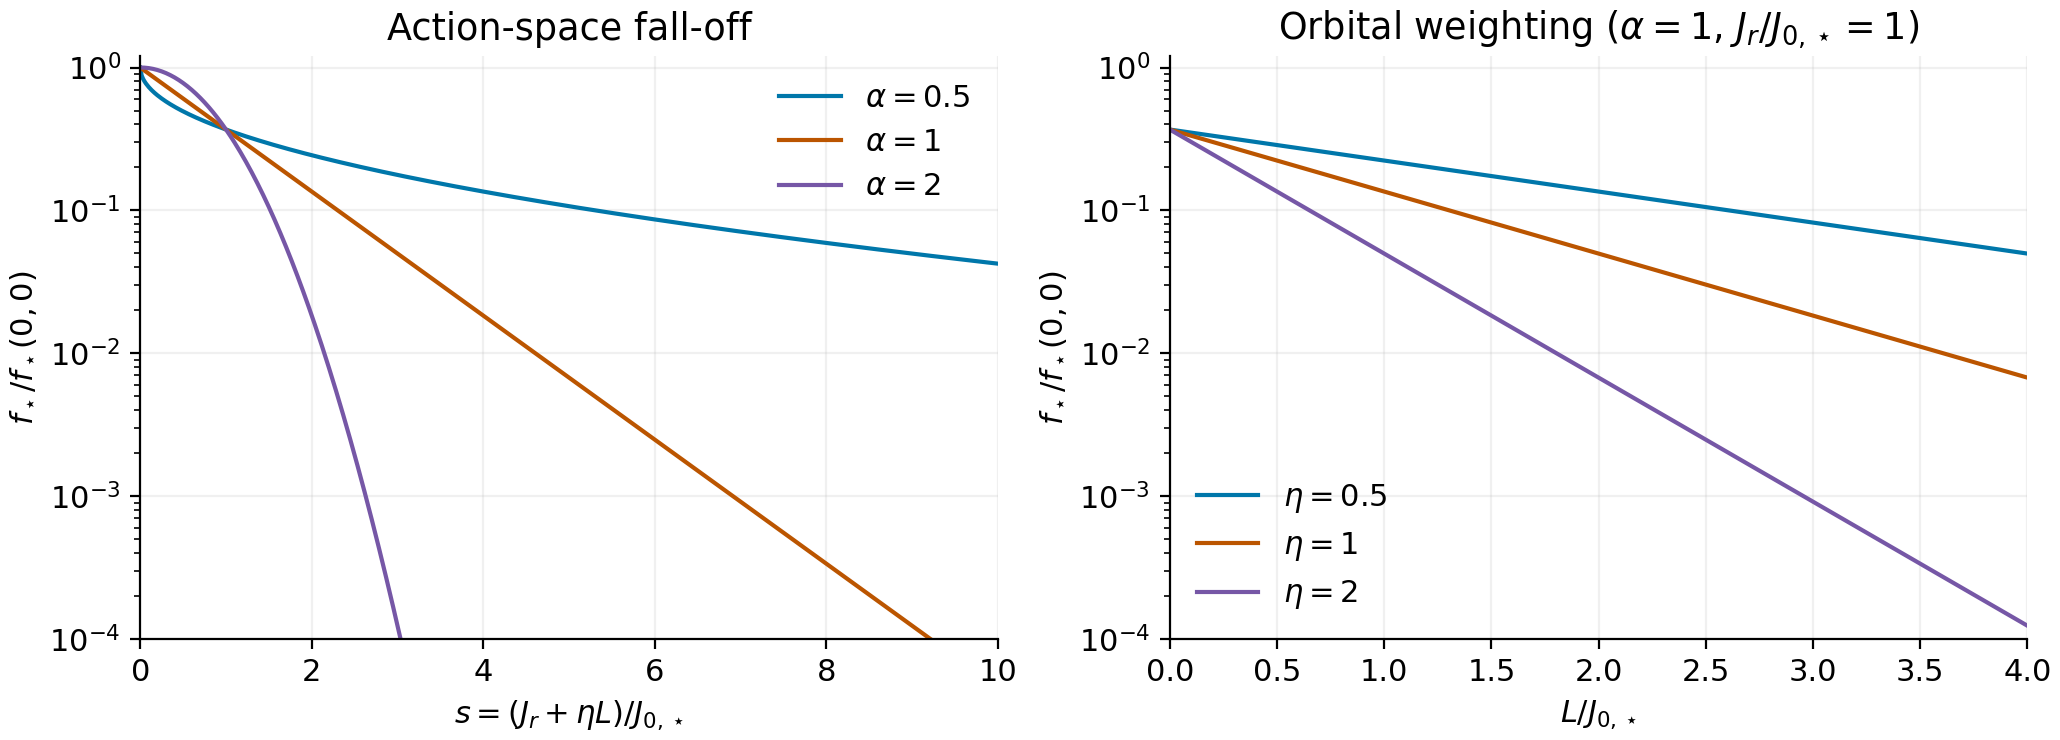
\includegraphics[width=\linewidth]{compact_df_proposal_action_shapes.png}
\caption{Analytic slices of the diagnostic precursor,
equation~\eqref{eq:precursor}, divided by their own zero-action values.
The different $\alpha$ and $\eta$ curves illustrate envelope and orbital
weighting; their mass-normalization constants differ. These are not density
profiles, $\beta(r)$ predictions or the proposed regularized DF.}
\label{fig:action}
\end{figure}
\FloatBarrier

\clearpage
\bibliographystyle{plainnat}
\bibliography{df_model_literature}
\end{document}
